\section{TKlog}

В этом разделе вводится новый тип подстановок TKlog, частным случаем которого является \(\pi\). Стрибог и Кузнечик были разработаны ''ТК-26''\footnote{Официальное название этой организации ''Технический Комитет По Стандартизации №26 «Криптографическая Защита Информации»''}, поэтому используется аббревиатура ''TK'' в TKlog. Она обладает логарифмическими свойствами, хотя и отображает \(\mathrm{GF}(2^{2m})\) в себя, а не в \(\mathbb{Z}/2^{2m}\mathbb{Z}\), отсюда и ''log'' в TKlog. Более точно, она отображает разложение \(\mathrm{GF}(2^{2m})\) на мультипликативные смежные классы \(\mathrm{GF}(2^m)^*\) в разбиение на аддитивные смежные классы \(\mathrm{GF}(2^m)\), и ее ограничение на каждый мультипликативный смежный класс класс по сути одинаково для всех смежных классов. Эта структура будет определена в Разделе 2.1, а в Разделе 2.2 будут представлены детали этого свойства, сохраняющего разбиение.

\subsection{Перестановочная структура TKlog}

\textbf{TKlog.} Пусть \(\mathrm{GF}(2^{2m}) = \mathbb{F}_2[X]/p(X)\) — конечное поле, заданное примитивным многочленом \(p\). Мультипликативная подгруппа \(\mathrm{GF}(2^{2m})^*\) циклична и задается порождающим элементом \(\alpha\), таким что \(p(\alpha) = 0\). В этом случае \(\alpha^{2m+1}\) является порождающим элементом мультипликативной подгруппы подполя \(\mathrm{GF}(2^m)\).

\textbf{Определение 1} \((TKlog)\). TKlog — это подстановка, действующая на элементах поля \(\mathrm{GF}(2^{2m}) = \mathbb{F}_2[X]/p(X)\) для некоторого примитивного многочлена \(p\) с корнем \(\alpha\). Она задается:
\begin{itemize}
    \item аффинной функцией \(\kappa : \mathbb{F}^m_2 \to \mathrm{GF}(2^{2m})\) такой, что любой \(x \in \mathrm{GF}(2^{2m})\) может быть записан как \(x = x_m \oplus \kappa(x_\kappa) \oplus \kappa(0)\) для некоторых \(x_m \in \mathrm{GF}(2^m)\) и \(x_\kappa \in \mathbb{F}^m_2\)\footnote{Эквивалентно, можно записать, что линейная часть отображения \(\kappa\), которая отображает \(y \in \mathbb{F}_2^m\) в \(\kappa(y) \oplus \kappa(0) \in \mathbb{GF}(2^{2m})\), отображает \(\mathbb{F}_2^m\) в векторное пространство в прямой сумме с подполем \(\mathbb{GF}(2^m)\).};
    \item подстановкой \(s\) над \(\mathbb{Z}/(2^m - 1)\mathbb{Z}\).
\end{itemize}

Соответствующий TKlog обозначается \(\mathscr{T}_{\kappa,s}\) и действует следующим образом:

$$
\begin{cases}
  \mathscr{T}_{\kappa, s}(0) & =\kappa(0), \\
  \mathscr{T}_{\kappa, s}\left(\left(\alpha^{2^m+1}\right)^j\right) & =\kappa\left(2^m-j\right), \text { для } 1 \leq j \leq 2^m-1, \\
  \mathscr{T}_{\kappa, s}\left(\alpha^{i+\left(2^m+1\right) j}\right) & =\kappa\left(2^m-i\right) \oplus\left(\alpha^{2^m+1}\right)^{s(j)}, \text { для } 0<i, 0 \leq j<2^m-1,
\end{cases}
$$ где тот факт, что \(1 \leq j \leq 2^m - 1\), а не \(0 \leq j < 2^m - 1\), когда \(x \in \mathrm{GF}(2^m)^*\), следует из неявного использования логарифма Фэнга и др. (см Алгоритм 3 в Приложении Б).

Чтобы убедиться в том, что пример TKlog, определенный выше, действительно является подстановкой, следует определить его обратную функцию TKexp. Она использует \(\Phi_\kappa: \text{GF}(2^{2m}) \rightarrow \mathbb{F}^m_2 \times \text{GF}(2^m)\), которая является аффинной подстановкой такой, что:

\[
\Phi_\kappa(\kappa(x) \oplus v) = (x, v)
\] для \((x, v) \in \mathbb{F}^m_2 \times \text{GF}(2^m)\). TKexp работает следующим образом:
$$
\left\{\begin{array}{l}
  \left(\mathscr{T}_{\kappa, s}^{-1} \circ \Phi_\kappa^{-1}\right)(0,0)=0, \\
  \left(\mathscr{T}_{\kappa, s}^{-1} \circ \Phi_\kappa^{-1}\right)(k, 0)=\alpha^{\left(2^m+1\right)\left(2^m-k\right)}, \\
  \left(\mathscr{T}_{\kappa, s}^{-1} \circ \Phi_\kappa^{-1}\right)(k, v)=\alpha^{2^m-k+\left(2^m+1\right) s^{-1}(j)} \text { где } j=\log _\alpha^{F L Y}(v) /\left(2^m+1\right) .
  \end{array}\right.
$$

Альтернативно, это может быть вычислено с использованием Алгоритма 4 (в Приложении Б).

\textbf{О вычитании} \((Substraction).\) Целочисленное вычитание на входе \(\kappa\) необходимо из-за того, что \(i \in \{1, \ldots, 2^m\}\), поэтому двоичное представление \(i\) не всегда помещается в \(m\) бит. Cледовательно, нужна небольшая функция, которая отображает \(\{1, \ldots, 2^m\}\) в \(\{0, \ldots, 2^{m - 1}\}\), поскольку случай \(i = 0\) обрабатывается отдельно. Естественным выбором, очевидно, было бы \(i \mapsto i - 1\), но в этом случае потребуется другая функция для случая, когда \(i = 0\). Действительно, поскольку используется логарифм FLY, получается \(j \in \{1, \ldots, 2^{m - 1}\}\) для \(i = 0\). Таким образом, нужно будет получать \(\kappa\) из двух различных функций в зависимости от того, будет ли \(i = 0\). С другой стороны, функция \(i \leftarrow 2^m - i\) отображает и \(\{1, \ldots, 2^m\}\) в \(\{0, \ldots, 2^m - 1\}\) и \(\{1, \ldots, 2^m - 1\}\) в себя, то есть она может использоваться в обоих случаях.

В рамках данной работы не удалось найти такую простую функцию, когда используется логарифм \(\log_{\alpha}^{\text{HN}}\).

\textbf{Частный случай} $\bm{\pi}$. S-блок \(\pi\) является экземпляром 8-битного TKlog. Для целей реализации будем отождествлять \(\text{GF}(2^8)\) с \(\mathbb{F}^8_2\), используя метод, описанный в Разделе 1.1. Когда \(\pi\) записывается в виде экземпляра TKlog, она использует следующие компоненты:

\begin{itemize}
    \item конечное поле \(\text{GF}(2^8) = \mathbb{F}_2[X]/p_{\text{min}}(X)\), где \(p_{\text{min}}(X) = X^8 \oplus X^4 \oplus X^3 \oplus X^2 \oplus 1\) и его корень \(\alpha\);
    \item аффинная функция \(\kappa\), отображающая \(\mathbb{F}^4_2\) в \(\mathbb{F}^8_2\) так, что \(\kappa(0) = 0\)x\(\text{FC}\) с линейной частью \(\Lambda\), определенной как
    \[
    \Lambda(1) = 12, \quad \Lambda(2) = 26, \quad \Lambda(4) = 24, \quad \Lambda(8) = 30,
    \] где числа записаны в шестнадцатеричном формате и где линейная функция \(\Lambda\) проверяет \(\{x_4 \oplus \Lambda(y), x_4 \in \text{GF}(2^4), y \in \mathbb{F}^4_2\} = \text{GF}(2^8)\);
    \item подстановка \(s\) из \(\mathbb{Z}/15\mathbb{Z}\), определенная в Таблице \ref{tab:tab1}.
\end{itemize}

\begin{table}    
  \caption{Таблица поиска для подстановки \(s\) над \(\mathbb{Z}/15\mathbb{Z}\)}
  \begin{tabular}{cccccccccccccccc}
    \hline$x$ & 0 & 1 & 2 & 3 & 4 & 5 & 6 & 7 & 8 & 9 & 10 & 11 & 12 & 13 & 14 \\
    \hline$s(x)$ & 0 & 12 & 9 & 8 & 7 & 4 & 14 & 6 & 5 & 10 & 2 & 11 & 1 & 3 & 13 \\
    \hline
  \end{tabular}
  \label{tab:tab1}
\end{table}

Разложение \(\pi\) с использованием этой структуры представлена в Алгоритме \ref{alg:alg01}. Реализация \(\pi\), основанная на этом алгоритме, приведена как скрипт на SAGE \cite{Dev17} в Приложении Д. Примечательно, что функция логарифма по умолчанию в SAGE — это \(\log_{\alpha}^{\text{FLY}}\), что упрощает реализацию функции.

В итоге действительно удалось получить структуру TKlog, сначала разложив \(\pi\), а затем обобщив найденную структуру. Краткое описание процесса реверс-инжиниринга приведено в Приложении В.

\begin{algorithm}[htp!]
    \KwData{$x \in \text{GF}(2^8)$}
    \eIf{$x = 0$} {
      return $\kappa(0)$\;
    }{
      $k = \log_{\alpha}^{\text{FLY}}(x)$\;
      $i \gets k \bmod 17$; \quad $j \gets k/17 $ \Comment*[r]{$x = \alpha^{i+17j}$}
      \eIf{$i = 0$} { 
        return $\kappa(16 - j)$ \Comment*[l]{$x \in \text{GF}(2^4)$; $i = 0 \Rightarrow j \in \{1, \ldots, 15\}$}
      }{
        return $\kappa(16 - i) \oplus (\alpha^{17})^{s(j)}$ \Comment*[r]{$i \neq 0$, поэтому $16 - i \neq 16$}
      }
    }
  \caption{Новое разложение \(\pi\)}
  \label{alg:alg01}
\end{algorithm}

\subsection{Смежные классы к смежным классам}

\subsubsection{Свойство сохранения разбиения}

Напомним, что \(\mathrm{GF}(2^m)^*\) это мультипликативная группа поля размерности \(2^m\) и что она является подгруппой группы \(\mathrm{GF}(2^{2m})^*\). Пусть \(\alpha\) является порождающим элементом мультипликативной группы поля \(\mathrm{GF}(2^{2m})^*\) таким, что \(\alpha^{2^m+1}\) является порождающим элементом мультипликативной группы поля \(\mathrm{GF}(2^m)^*\). Поле \(\mathrm{GF}(2^{2m})\) можно представить двумя различными способами с использованием мультипликативных классов смежности по \(\mathrm{GF}(2^m)^*\) с одной стороны и аддитивных классов смежности с другой:

\begin{itemize}
  \item Все элементы \(\mathrm{GF}(2^{2m})^*\) можно представить в виде \(\alpha^{i+(2^m+1)j} = \alpha^i (\alpha^{2^m+1})^j\), так что
  \[
  \mathrm{GF}(2^{2m}) = \{0\} \cup \left(\bigcup_{i=0}^{2^m} \alpha^i \odot \mathrm{GF}(2^m)^*\right) = \mathrm{GF}(2^m) \cup \left(\bigcup_{i=1}^{2^m} \alpha^i \odot \mathrm{GF}(2^m)^*\right).
  \]
  \item Поскольку \(\mathrm{GF}(2^m)\) является векторным пространством размерности \(m\), существует векторное пространство \(W\) с элементами из \(\mathrm{GF}(2^{2m})\) размерности \(m\) такое, что \(\mathrm{GF}(2^{2m})\) является прямой суммой \(W\) и \(\mathrm{GF}(2^m)\). В этом случае можно записать
  \[
  \mathrm{GF}(2^{2m}) = \bigcup_{w \in W} w \oplus \mathrm{GF}(2^m) = W \cup \left(\bigcup_{w \in W} w \oplus \mathrm{GF}(2^m)^*\right).
  \]
\end{itemize}

\(W\) и \(\mathrm{GF}(2^m)\) являются векторными пространствами размерности \(m\), и в каждом разложении используется \(2^m\) классов смежности \(\mathrm{GF}(2^m)^*\). Следовательно, можно отобразить эти разложения друг в друга. Это как раз то, что делает TKlog. Более формально это будет рассмотрено в Теореме 1.

\textbf{Теорема 1}. Пусть \(\mathscr{T}_{\kappa,s} : \mathrm{GF}(2^{2m}) \to \mathrm{GF}(2^{2m})\) является экземпляром TKlog. Тогда верны следующие равенства:
\[
\begin{cases}
  \mathscr{T}_{\kappa,s}(\mathrm{GF}(2^m)) & = \kappa(\mathbb{F}_2^m) \\
  \mathscr{T}_{\kappa,s}(\alpha^i \, \odot \, \mathrm{GF}(2^m)^*) & = \kappa(2^m - i) \oplus \mathrm{GF}(2^m)^*, \forall i \neq 0.
\end{cases}
\]

\textbf{Следствие 1}. Пусть \(\mathscr{T}_{\kappa,s} : \mathrm{GF}(2^{2m}) \to \mathrm{GF}(2^{2m})\) является допустимым экземпляром TKlog. Тогда верно, что
\[
  \mathscr{T}_{\kappa,s}(\mathrm{GF}(2^m)) = \kappa(\mathbb{F}_2^m) \text{ и } \mathscr{T}_{\kappa,s}(\alpha^{2^m} \odot \mathrm{GF}(2^m)) = \kappa(0) \oplus \mathrm{GF}(2^m),
\] где все пространства имеют размерность \( m \). Кроме того,
\begin{align*}
GF(2^{2m}) & = \{ x \oplus y, x \in GF(2^m), y \in \alpha^{2m} \odot GF(2^m) \} \\
& = \{ x \oplus y, x \in \kappa(0) \oplus GF(2^m), y \in \kappa(0) \oplus \kappa (\mathbb{F}_{2}^{m}) \},
\end{align*}
таким образом, \( \text{TKlog} \) отображает два векторных пространства размерности \( m \) в два аффинных пространства размерности \( m \).

Поскольку \( \pi \) является экземпляром TKlog, из Теоремы 1 следует, что она проверяет следующее равенство множеств:
\[
  \begin{cases}
\pi\left( GF(2^4) \right) & = \kappa(\mathbb{F}_{2}^{4}) \\
\pi\left( \alpha^i \odot GF(2^4)^{\ast} \right) & = \kappa(16 - i) \oplus GF(2^m)^{\ast}, \quad \forall i \neq 0,
  \end{cases}
\]
и применение Следствия 1 дает \(\pi(\alpha^{16} \odot GF(2^4)) = \kappa(0) \oplus GF(2^4)\). Эти равенства продемонстрированы на Рисунке \ref{fig:fig02}, где связи между полными аффинными пространствами представлены пунктирными стрелками, а связи между множествами размерности \(2^m - 1\) представлены сплошными стрелками.

\begin{figure}
  \centering
  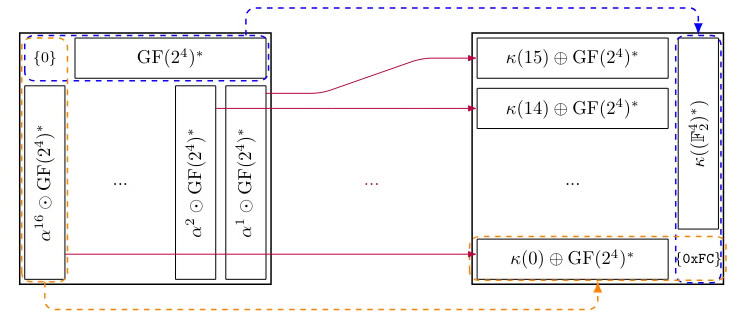
\includegraphics[scale=0.7]{contents/pics/cosets.png}
  \caption{Разбиение $GF(2^8)$ на мультипликативные смежные классы по $GF(2^4)^*$ (слева), аддитивные смежные классы по $GF(2^4)^*$ (справа) и действие $\pi$ на них (стрелки)}
  \label{fig:fig02}
\end{figure}

\subsubsection{Простота свойств TKlog}
Разбиения, рассматриваемые в Теореме 1, имеют простые алгебраические описания. Действительно,
\( x, y \in GF(2^{2m})^{\ast} \) принадлежат одному и тому же аддитивному смежному классу \( GF(2^m)^{\ast} \), тогда и только тогда, когда выполнено равенство \( \text{Tr}_m(x) = \text{Tr}_m(y) \).
Отметим, что
\[
\left(\alpha^{i+(2m+1)j}\right)^{2^m-1} = \alpha^{(2^m-1)i+(2^{2m}-1)j} = \alpha^{(2^m-1)i},
\]
таким образом, $\left(\alpha^{i+(2m+1)j}\right)^{2^m-1} = \left(\alpha^{i'+(2m+1)j'}\right)^{2^m-1}$ тогда и только тогда, когда \( i = i' \). Следовательно, \( x, y \in GF(2^{2m})^{\ast} \) принадлежат одному и тому же мультипликативному смежному классу \( GF(2^m)^{\ast} \) тогда и только тогда, когда \( x^{2^m-1} = y^{2^m-1} \). Кроме того, \( x \in GF(2^m)^{\ast} \) тогда и только тогда, когда \( x^{2^m-1} = 1 \). Таким образом получается еще одно следствие Теоремы 1.

\textbf{Следствие 2.} Пусть \( \mathscr{T}_{\kappa,s} : GF(2^{2m}) \to GF(2^{2m}) \) является экземпляром TKlog. Тогда:
\[
x^{2^m-1} = y^{2^m-1} \neq 1 \Leftrightarrow \text{Tr}_m(\mathscr{T}_{\kappa,s}(x)) = \text{Tr}_m(\mathscr{T}_{\kappa,s}(y)) \neq \text{Tr}_m(\kappa(0)).
\]

Как следствие, для любой константы \( c \in GF(2^{2m}) \setminus \{0, 1\} \), получается следующее следствие, включающее только линейные уравнения:
\[
x^{2^m} \oplus cx = y^{2^m} \oplus cy = 0 \implies (\mathscr{T}_{\kappa,s}(x))^{2^m} \oplus \mathscr{T}_{\kappa,s}(x) = (\mathscr{T}_{\kappa,s}(y))^{2^m} \oplus \mathscr{T}_{\kappa,s}(y).
\]

Взаимодействие TKlog с этими двумя разбиениями выходит за рамки отображения одного в другое. Действительно, рассмотрим более общую структуру, соответствующую подстановкам \( P \) таким, что:
\begin{equation}
  P :
  \begin{cases}
    0 & \mapsto \kappa (t_0(0)) \\
    \alpha^{(2m+1)j} & \mapsto \kappa (t_0(2^m - j)) \\
    \alpha^{i+(2m+1)j} & \mapsto \kappa (t_1(2^m - i)) \oplus (\alpha^{2m+1})^{s_i(j)} \text{ для } i > 0,
  \end{cases}
  \label{eq:02}
\end{equation}
где \( t_0 \) и \( t_1 \) являются подстановками над \( \mathbb{F}_{2}^{m} \), и где \( s_i \) является подстановкой над \( \mathbb{Z}/(2^m - 1)\mathbb{Z} \) для всех \( i \in \mathbb{Z}/(2m + 1)\mathbb{Z} \). Любая такая \( P \) является подстановкой с точным свойством сохранения разбиения, описанного в Теореме 1, но ее вклад в \( GF (2^m) \) и в \( \kappa(\mathbb{F}_{2}^{m}) \) зависит от \( i \) и \( j \), даже если рассматривать только случай \( i > 0 \). В случае с TKlog это не так. Эти подстановки намного проще.

\textbf{Лемма 1} \textit{(Свойство разбиения).} Пусть \( \mathscr{T}_{\kappa,s} : GF(2^{2m}) \to GF(2^{2m}) \) является экземпляром TKlog. Тогда для любых \( i, j \), таких что \( 0 < i \leq 2^m \) и \( 0 \leq j < 2^m - 1 \), выполняется:
\[
  \mathscr{T}_{\kappa, s}\left(\alpha^{i+\left(2^m+1\right) j}\right)=\underbrace{\kappa\left(2^m-i\right)}_{\in \kappa\left(F_2^m\right)} \oplus \underbrace{\left(\alpha^{2^m}+1\right.}_{\in \mathrm{GF}\left(2^m\right)^*})^{s(j)},
\]
так, что вклад \( i \) ограничен \( \kappa(\mathbb{F}_{2}^{m}) \), а вклад \( j \) ограничен \( GF(2^m) \).

Другими словами, TKlog взаимодействует с каждым мультипликативным смежным классом, отличным от \( GF(2^m)^{\ast} \), совершенно одинаково, хотя это свойство никак не вытекает из Теоремы 1.

В рамках данной работы не удалось обнаружить ни одной атаки, использующей эти свойства \( \pi \). Однако было обнаружено, что эти разбиения взаимодействуют нетривиальным образом с линейным слоем алгоритма Стрибог. Последствия наличия этой структуры в \( \pi \) будут рассмотрены в Разделе 4.